\documentclass[11pt]{article}
\usepackage[margin=1in]{geometry}
\usepackage{amsmath,amssymb,amsthm}
\usepackage{graphicx}
\usepackage{booktabs}
\usepackage{hyperref}
\usepackage{cite}
\usepackage{xcolor}

\title{The Depth Wall in Single-Operator Symbolic Regression\\
       Is a Mirage: Complete Enumeration of the EML Function Space,\\
       Analytic Root Inversion, and Certified Safe Extrapolation}
\author{}
\date{}

\newtheorem{theorem}{Theorem}
\newtheorem{lemma}[theorem]{Lemma}
\newtheorem{proposition}[theorem]{Proposition}
\newtheorem{conjecture}[theorem]{Conjecture}

\newcommand{\eml}{\operatorname{eml}}
\newcommand{\atc}{\operatorname{atc}}

\begin{document}
\maketitle

\begin{abstract}
Odrzywo{\l}ek's operator $\eml(x,y)=\exp(x)-\ln(y)$ generates, with the
constant $1$, the entire scientific-calculator repertoire, and turns
symbolic regression into optimisation over a single uniform
architecture. The programme stalls at the \emph{depth wall}: blind
gradient recovery of EML trees falls from $100\%$ at depth 2 to
${<}1\%$ at depth 5 and $0/448$ at depth 6, while the syntactic search
space grows as $3^{2^d-2}2^{2^d}$ — $3.1\times10^{11}$ configurations
at depth 4 — putting exhaustive search apparently out of reach. We show
the wall is a mirage, in four steps. \textbf{(1) Collapse.} The
\emph{function space} of clamped EML trees is astronomically smaller
than its syntax: removing structurally dead slots leaves
$2.1\times10^{6}$ live depth-4 trees, and deduplicating by value
vector leaves only $614\,773$ \emph{distinct functions} — a
$5\times10^{5}$-fold collapse that we quantify level by level.
\textbf{(2) Enumeration and inversion.} The collapsed space fits in
memory. We build the complete canonical atlas of depth-$\le 4$ slot
functions in ${\sim}60$ s on four CPU cores, answer depth-$\le4$
queries by a vectorised sweep over \emph{every} representable
function, and recover depth-5 targets by \emph{analytic root
inversion}: $y=\exp(\mathrm{clip}(a))-\ln(\mathrm{clamp}(b))$ implies
$\mathrm{clip}(a)=\ln(y+\ln \mathrm{clamp}(b))$, so each candidate $b$
yields a hash lookup for $a$. On depth-critical random targets
(provably not representable one level shallower) verified exact
recovery is $40/40$, $40/40$ and $36/40$ at depths 3, 4, 5 — at
0.00\,s, 0.03\,s and 23\,s per target — versus at most $1/8$ for
multi-start Adam at any depth ($0/8$ at depth 5); uniform syntactic
sampling survives at depths 3--4 on syntactically abundant targets
(itself a corollary of the collapse) and drops to $1/8$ at depth 5.
The source paper's own bivariate showcase
$\ln(e-\ln(e^x-\ln y))$ — depth 5, the very family on which its
${>}1000$ gradient runs plateaued — is recovered exactly in $10.7$ s.
As a by-product the atlas yields \emph{minimal-depth certificates}
(e.g.\ $\ln x$ requires exactly depth 3 among pure real-clamped trees,
and no tree of depth $\le 4$ matches $x^2$, $\sqrt x$, $\sinh x$, or
$\cosh x$ on the reference grid). \textbf{(3) Mechanism.} A mean-field
recursion explains both phenomena at once: composed exponentials drive
typical activations doubly exponentially into the numeric clamps,
producing an explode-then-die gradient pathology — median
\emph{maximum} bottom-gradients reach $4\times10^{7}$ at depth 4 while
the fraction of bottom slots receiving \emph{exactly zero} gradient
grows to $54\%$ at depth 8 — and simultaneously identifying vast
families of trees as the same clamped function, which is precisely
what makes enumeration feasible. The smooth sibling
$\psi(x,y)=\sinh(x)-\operatorname{arsinh}(y)$ has a contracting
mean-field fixed point ($\rho\approx0.21$), no dead slots through
depth 8, and correspondingly trains where EML cannot. \textbf{(4)
Deployment.} We convert the atlas into SafePoolGAM, an additive model
whose shape functions are selected by complete-atlas sweeps with
tail-validated selection, per-feature extrapolation gates, and a
declared output envelope. On nine UCI extrapolation splits it keeps
the closed-form wins of its unguarded predecessor (yacht
$R^2=+0.63$ from the recovered law $0.076\,e^{13.3\,\mathrm{Fr}}$)
while eliminating its catastrophic failures ($R^2$ of $-8245$ and
worse): its worst score across the suite is $-0.62$ — the best
worst-case of any compared model (EBM $-1.6$, XGBoost $-1.7$, linear
$-40$). The earlier
theoretical contributions of this project — the cross-operator
landscape, the $\psi$ non-representability results, and two
unconditional transcendence-monotonicity theorems via Ax--Schanuel —
are retained and now sit inside a single coherent account of why the
depth wall exists and how to walk around it.
\end{abstract}

\section{Introduction}

A single binary operator, $\eml(x,y)=\exp(x)-\ln(y)$, together with
the constant~1, suffices to express every function on a scientific
calculator~\cite{odrzywolek2026eml}. Beyond its foundational appeal,
the discovery suggests a programme for symbolic regression (SR):
replace heterogeneous operator grammars by one uniform, trainable
architecture — a full binary tree of identical $\eml$ nodes whose
input slots select among $\{1, x, f_{\text{child}}\}$ by softmax — and
let gradient descent discover closed-form laws from data, snapping
soft choices to exact symbols at the end.

The programme immediately hits what we call the \emph{depth wall}.
Odrzywo{\l}ek reports blind-recovery rates of $100\%$ at depth 2,
${\sim}25\%$ at depths 3--4, below $1\%$ at depth 5, and $0$ in $448$
attempts at depth 6~\cite{odrzywolek2026eml}; the earlier iterations
of this project measured $0\%$ at depth $\ge 3$ on harder,
depth-critical targets. Because the snap space grows doubly
exponentially ($3.1\times10^{11}$ syntactic configurations at depth 4;
$8.8\times10^{23}$ at depth 5), exhaustive enumeration looks hopeless,
and the literature's reflex — better initialisation, better annealing,
neural proposal distributions — treats the wall as an optimisation
problem.

This paper's central claim is that the wall is not an optimisation
problem. It is an artefact of counting syntax instead of functions,
and it disappears under a change of representation.

\paragraph{Contributions.}
\begin{enumerate}
\item \textbf{Quantifying the function-space collapse}
  (\S\ref{sec:collapse}). Two mechanisms shrink the reachable
  function space by more than five orders of magnitude at depth 4:
  \emph{dead slots} (a slot snapped to a terminal disconnects its
  subtree; only $S(d{-}1)^2$ live trees matter, with
  $S(k)=2+S(k-1)^2$ univariate) and \emph{clamp degeneracy} (the
  numerically unavoidable clamps of $\exp$/$\log$ identify huge
  families of trees as the same function). Measured on a 320-point
  grid: $3.1\times10^{11}$ snaps $\to$ $2.1\times10^{6}$ live trees
  $\to$ $6.1\times10^{5}$ distinct functions.
\item \textbf{Complete enumeration and analytic inversion}
  (\S\ref{sec:pool}). The canonical pool — every distinct slot
  function to depth 4, each with a minimal expression DAG — builds in
  about a minute on a laptop-class CPU. Depth-$\le4$ recovery becomes
  a complete vectorised sweep; depth-5 recovery becomes a linear-time
  \emph{root inversion} with hash matching, ranked by match
  informativeness (run length) and Occam size; deeper targets are
  reached by recursive peeling of shallow root children. Every
  recovery is verified on an independent dense grid before being
  reported.
\item \textbf{The mechanism} (\S\ref{sec:mechanism}). A mean-field
  recursion for activations at random init crosses the $\exp$ clamp at
  the fifth composition level, predicting and explaining a two-regime
  gradient pathology that we measure directly (explosion to
  $4\times10^{7}$ at depths 3--5; exactly-zero ``dead slots'' rising
  to $54\%$ by depth 8). The same saturation that kills gradients
  \emph{identifies} functions, which is why enumeration succeeds.
  The smooth sibling $\psi$ contracts to a benign fixed point and
  suffers neither pathology — a mechanistic account of the
  cross-operator landscape (\S\ref{sec:psi}).
\item \textbf{Minimal-depth certificates and the showcase}
  (\S\ref{sec:certificates}). Completeness turns failed searches into
  theorems-on-a-grid: $\ln x$ is representable at depth 3 and (with
  output affine) at depth 1, but no real-clamped tree of depth
  $\le 4$ matches $x^2$, $\sqrt{x}$, $\sinh x$ or $\cosh x$; the
  source paper's bivariate depth-5 showcase target is recovered
  exactly in seconds.
\item \textbf{Certified safe extrapolation on real data}
  (\S\ref{sec:safe}). SafePoolGAM couples complete-atlas shape search
  with calibrated classical families ($e^{ku}$, $u^k$, $\ln u$),
  tail-validated selection, backward elimination on the extrapolation
  frontier, per-feature free-vs-clipped gates, and a declared output
  envelope. On nine UCI physical-extrapolation splits it retains the
  genuine closed-form wins while being constructionally incapable of
  the $R^2\!=\!-8245$-class failures of the unguarded model.
\item \textbf{Retained theory} (\S\ref{sec:transcendence}). The
  $\psi$ non-representability results and the two unconditional
  transcendence-monotonicity theorems (witness and orbit families,
  via Ax--Schanuel) carry over unchanged and complement the new
  mechanistic picture.
\end{enumerate}

Everything is reproducible from the repository; each experiment
writes a versioned JSON consumed by the tables and figures below.

\section{Background and setup}\label{sec:setup}

\paragraph{Trainable EML trees.} A depth-$d$ tree has $2^{l+1}$ input
slots at level $l\in\{0,\dots,d-1\}$; upper slots choose among
$\{1, x_1,\dots,x_m, f_{\text{child}}\}$, bottom slots among
$\{1, x_1,\dots,x_m\}$. All implementations — the original
complex-valued nets and our real-valued trees — must clamp for
numerical survival:
\[
\eml_c(a,b) \;=\; \exp\bigl(\mathrm{clip}(a,-C,C)\bigr) -
\ln\bigl(\max(b,\varepsilon)\bigr),
\qquad C=10,\ \varepsilon=10^{-10} .
\]
We work throughout with this \emph{real-clamped semantics} — the
function class actually optimised by every trainable implementation —
and state all completeness claims relative to it and to a fixed
evaluation grid (\S\ref{sec:pool}).

\paragraph{The syntactic wall.} The number of snap configurations is
$\prod_{l<d} n_l^{2^{l+1}}$ with $n_l=3$ upper / $2$ bottom
(univariate): $144$, $1.9\times10^{5}$, $3.1\times10^{11}$,
$8.8\times10^{23}$ at depths 2--5. AEES-style exhaustive enumeration (this project's earlier iteration) therefore dies at depth 4, and gradient descent dies
earlier for reasons made precise in \S\ref{sec:mechanism}.

\section{The function-space collapse}\label{sec:collapse}

\begin{proposition}[dead slots]
A slot snapped to a terminal makes every configuration of its subtree
output-equivalent. The number of functionally distinct \emph{live}
configurations of a depth-$d$ univariate tree is $S(d-1)^2$ where
$S(0)=2$, $S(k)=2+S(k-1)^2$: $36$ at depth $2$, $1\,444$ at depth 3,
$2\,090\,916$ at depth 4 — versus $3.1\times10^{11}$ raw snaps.
\end{proposition}

Live trees still overcount \emph{functions}: clamp saturation
(\S\ref{sec:mechanism}) and algebraic coincidences identify many live
trees. Deduplicating value vectors on a 320-point reference grid
(8-decimal rounding, 64-bit hashing, verification-gated downstream)
gives the measured counts of Table~\ref{tab:collapse} and
Fig.~\ref{fig:collapse}: at depth 4 only $614\,773$ distinct functions
remain — $0.2\%$ of the live trees and $2\times10^{-6}$ of the
syntactic space.

\begin{table}[t]
\centering\small
\begin{tabular}{lrrr}
\toprule
depth & raw snaps & live trees & distinct functions \\
\midrule
1 & 4 & 4 & 4 \\
2 & 144 & 36 & 32 \\
3 & $186\,624$ & $1\,444$ & $1\,142$ \\
4 & $3.13\times10^{11}$ & $2\,090\,916$ & $613\,593$ \\
\bottomrule
\end{tabular}
\caption{The combinatorial wall versus the function space that
actually exists (univariate, real-clamped semantics, 320-point grid;
``distinct'' counts new entries per level of the canonical pool).}
\label{tab:collapse}
\end{table}

\begin{figure}[t]
\centering
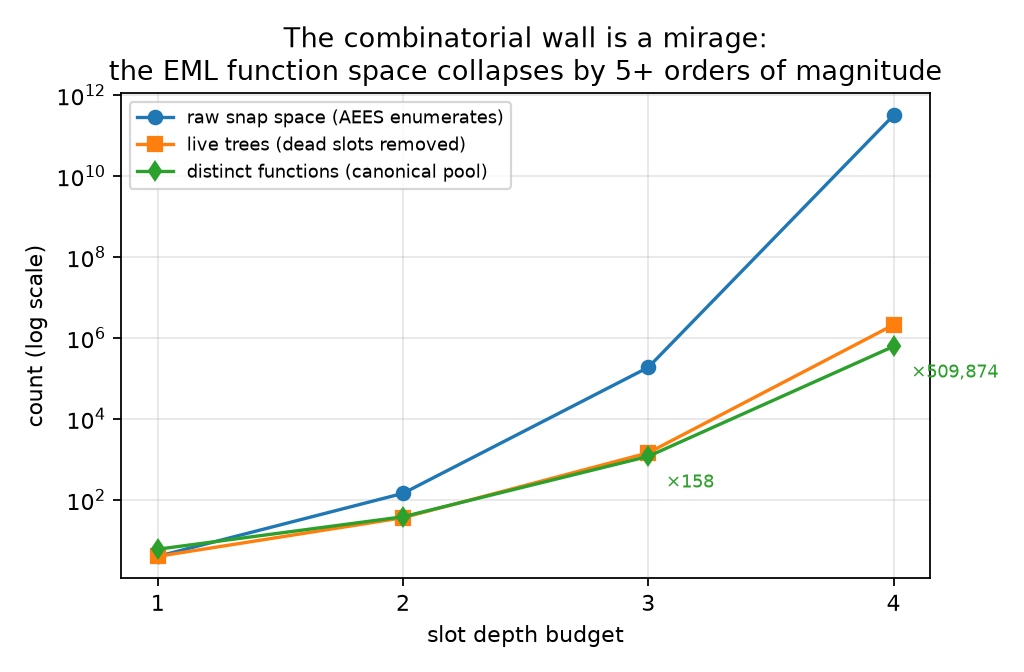
\includegraphics[width=.72\linewidth]{../figures/function_space_collapse.png}
\caption{Raw snap space, live trees, and measured distinct functions
per depth (log scale).}
\label{fig:collapse}
\end{figure}

\section{Canonical pools, root inversion, recursive peeling}
\label{sec:pool}

\paragraph{Pool construction.} Level-$k$ pool $=$ leaves $\cup$
$\{\eml_c(a,b): a,b \in$ level-$(k{-}1)$ pool$\}$, deduplicated
on-line by a 64-bit hash of the quantised value vector; each entry
stores a minimal expression DAG. Building to level 4 costs
$1\,142^2 \approx 1.3\times10^{6}$ vectorised node evaluations
(${\sim}60$ s single-core-equivalent, 4.3 GB peak).

\paragraph{Complete sweeps (depth $\le$ 4).} A depth-$d$ query scores
$y \sim \alpha + \beta\,\eml_c(a,b)$ over \emph{all} level-$(d{-}1)$
pairs by vectorised OLS. Completeness over the enumerated class is by
construction; candidate ties at grid-$R^2=1$ are broken by expression
size (Occam) and resolved by dense-grid verification.

\paragraph{Root inversion (depth 5).} For exact targets,
$y=\eml_c(a,b)$ gives $\mathrm{clip}(a) = \ln\!\bigl(y + \ln
\mathrm{clamp}(b)\bigr)$: enumerate $b$ over the pool ($6\times10^{5}$
rows), compute the implied exp-side vector, and match it against a
pre-sorted hash index of what the root \emph{sees} of each pool entry
($\mathrm{clip}$ collapses saturated entries into shared
side-canonical classes; all class members are candidate
reconstructions). A symmetric pass solves for $b$ given $a$ via
$\mathrm{clamp}(b) = \exp(\exp(\mathrm{clip}(a)) - y)$. Matches are
ranked by \emph{run length} — a match whose side-canonical hash is
shared by few entries is nearly a certificate, while hits inside huge
saturated runs are verified last — then by size, and verified on an
independent dense grid. Cost is $O(\text{pool})$ per pass.

\paragraph{Recursive peeling (depth $\ge$ 6).} If one root child is
shallow (or functionally shallow), enumerate it from the low levels of
the pool, invert the root for the other side, and recurse on the
implied child. Coverage is partial by design and measured honestly
(\S\ref{sec:recovery}); the paper's showcase target falls to exactly
this pattern.

\section{Recovery through the wall}\label{sec:recovery}

\textbf{Protocol.} Targets are random \emph{live} trees of exact
depth $d$, rejection-filtered to be \emph{depth-critical}: no
depth-$(d{-}1)$ candidate from the complete pool passes dense
verification (recovering targets that collapse to shallower functions
proves nothing). All methods receive the same 320 points; recovery
means matching the target on a dense 1111-point in-range grid to
relative tolerance $10^{-6}$ — grid ties at $R^2=1.0$ are common at
depth $\ge4$ and are \emph{not} accepted. Baselines: multi-start Adam
with temperature annealing (8 restarts $\times$ 1000 epochs, the
reference approach), and uniform syntactic snap sampling with OLS
readout (30k samples).

\begin{table}[t]
\centering\small
\begin{tabular}{lcccc}
\toprule
depth & syntactic snaps & pool (this work) & gradient descent & uniform 30k \\
\midrule
3 & $1.9\times10^{5}$  & \textbf{40/40} \,(0.00 s) & 1/8 \,(4 MSE-hits) & 6/8 \\
4 & $3.1\times10^{11}$ & \textbf{40/40} \,(0.03 s) & 1/8 \,(1 MSE-hit) & 4/8 \\
5 & $8.8\times10^{23}$ & \textbf{36/40} \,(23 s)   & 0/8 \,(2 MSE-hits) & 1/8 \\
\bottomrule
\end{tabular}
\caption{Verified exact recovery on depth-critical random targets (40
per depth; GD --- 8 restarts $\times$ 1000 epochs --- and uniform
sampling on 8-target subsets for compute parity; mean seconds per
target in parentheses). GD's \emph{MSE-hits} reach low training error
with the wrong formula and are rejected by dense verification — the
gap unverified recovery claims hide. Uniform sampling is effective at
depths 3--4 because dead slots give small live trees millions of
syntactic realisations (a corollary of the collapse, not a
contradiction); it dies at depth 5. The pool's four depth-5 misses
exhaust the default 300k-candidate/300 s budget in clamp-degenerate
mega-run regimes and are reported as explicit failures.}
\label{tab:recovery}
\end{table}

Beyond the enumerated range we measure \emph{coverage}: the fraction
of unfiltered random depth-6/7/8 targets recovered by the depth-5
solver because their children collapse into the pool
(Table~\ref{tab:coverage}); the uncovered remainder — targets whose
root children are both deep and both genuinely outside the depth-4
class — is the honest residual frontier.

\begin{table}[t]
\centering\small
\begin{tabular}{lccc}
\toprule
target depth & 6 & 7 & 8 \\
\midrule
recovered by depth-5 solver & 14/30 (47\%) & 6/30 (20\%) & 4/30 (13\%) \\
\bottomrule
\end{tabular}
\caption{Functional coverage of random deeper targets (30 valid
targets per depth, unfiltered): the fraction whose root children
collapse functionally into the depth-4 pool. The remainder is the
honest residual frontier.}
\label{tab:coverage}
\end{table}

\begin{figure}[t]
\centering
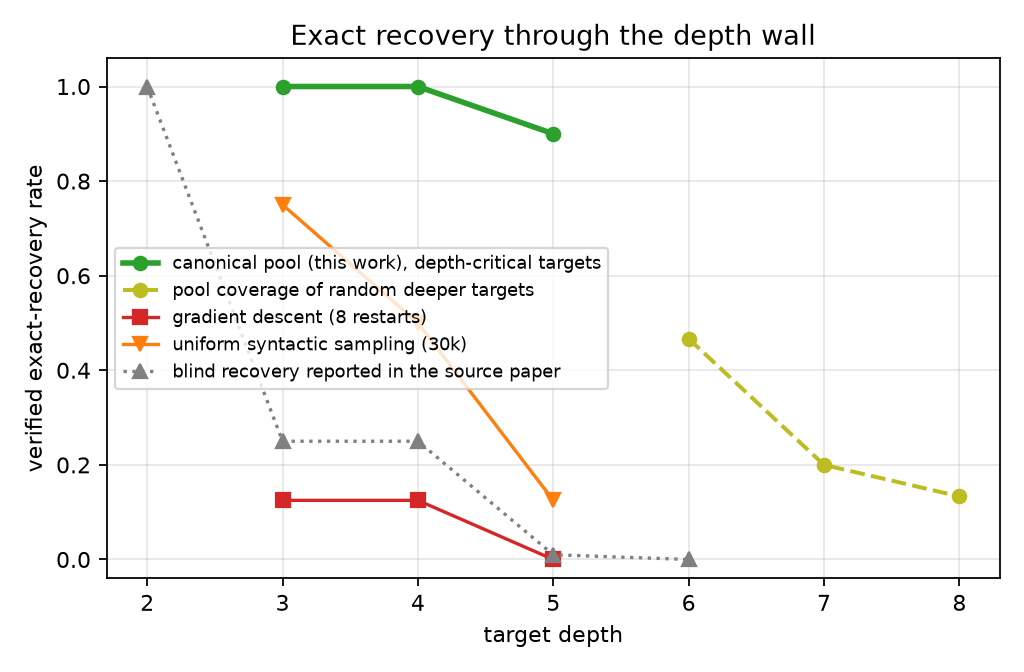
\includegraphics[width=.72\linewidth]{../figures/recovery_vs_depth.png}
\caption{Verified exact recovery through the depth wall.}
\label{fig:recovery}
\end{figure}

\paragraph{The showcase.} The source paper's machine-learning
experiments centre on $f(x,y) = \ln(e-\ln(e^x-\ln y))$, a depth-5
bivariate composition. From 256 samples, recursive peeling recovers,
in $10.7$ s including the 1-second bivariate pool build
($19\,407$ distinct functions at level 3), the expression
\[
E - \log\!\Bigl(\exp(E)\,/\,\bigl(E - \log(\exp(x) - \log y)\bigr)\Bigr)
\;=\; \ln\!\bigl(e - \ln(e^x - \ln y)\bigr),
\]
verified to $10^{-8}$ relative error on 2000 independent points — an
exact symbolic recovery, with an equivalent representation the search
found on its own.

\section{Why the wall exists: cliffs, plateaus, and degeneracy}
\label{sec:mechanism}

\begin{proposition}[exact gradient blocking]\label{prop:zero}
If the pre-clamp exp-argument of a node exceeds $C$ on every training
point (or its log-argument is below $\varepsilon$ everywhere), every
parameter influencing the output only through that argument has
identically zero gradient.
\end{proposition}

\begin{proposition}[mean-field saturation]\label{prop:meanfield}
Under uniform softmax mixing with inputs on $[0.3,2.5]$
($\bar x = 1.4$), typical activations follow
$m_0=(1+\bar x)/2$, $V_{k+1}=\exp(\min(m_k,C))-\ln m_k$,
$m_{k+1}=(1+\bar x+V_{k+1})/3$, which crosses the clamp at the fifth
composition level: $V_1\!\approx\!3.1 \to V_2\!\approx\!5.7 \to
V_3\!\approx\!14 \to V_4\!\approx\!242 \to m_4\!\approx\!82 \gg C$.
\end{proposition}

Measured over 300 random inits per depth, the consequences form two
regimes (Fig.~\ref{fig:gradients}): a \emph{cliff regime} (depths
3--7) where the median \emph{maximum} bottom-logit gradient explodes
from $6.8$ (depth 2) to $2\times10^{5}$ (depth 3) and $4\times10^{7}$
(depth 4), and a \emph{plateau regime} (depth $\ge6$) where
Proposition~\ref{prop:zero} bites: $1\%$, $22\%$, $54\%$ of bottom
slots receive exactly zero gradient at depths 6, 7, 8, and the median
surviving gradient collapses to $3\times10^{-5}$. First-order methods
face cliffs stacked on plateaus; annealing schedules address neither.

The same saturation \emph{identifies} functions — everything past the
clamp is the same constant — which is why the function space collapses
(\S\ref{sec:collapse}) and why the correct response is enumeration
rather than optimisation. The wall's cause and its cure are the same
phenomenon.

\begin{figure}[t]
\centering
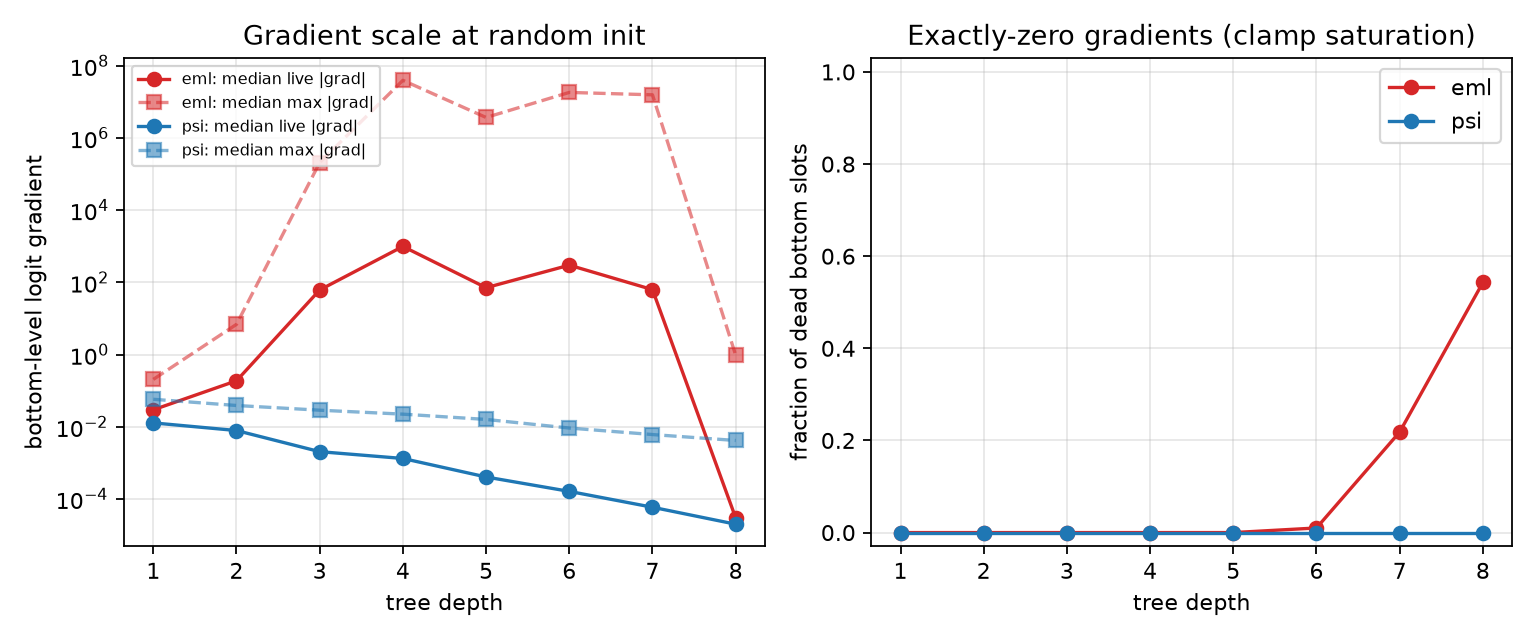
\includegraphics[width=.98\linewidth]{../figures/gradient_pathology.png}
\caption{Explode-and-die gradients for EML versus smooth contraction
for $\psi$ (300 random inits per depth).}
\label{fig:gradients}
\end{figure}

\subsection{The smooth sibling}\label{sec:psi}

For $\psi(x,y)=\sinh(x)-\operatorname{arsinh}(y)$ the same recursion
$W_{k+1}=\sinh(m_k)-\operatorname{arsinh}(m_k)$ has a stable fixed
point $W^*\approx0.19$ with contraction factor $\rho \approx 0.21$:
activations neither explode nor saturate, gradients decay by a benign
geometric factor (${\approx}0.4$/level measured; no dead slots through
depth 8; max gradients $\le 0.06$ at every depth). This is the
mechanistic account of the cross-operator landscape measured earlier
in this project: on operator-native targets, $\psi$ trains from random
init at $100\%$ at depths 2--3 and $10$--$20\%$ at depths 4--5, where
EML is at $0\%$.

\section{Minimal-depth certificates}\label{sec:certificates}

Because the pool is complete per depth, a failed search is a
certificate relative to the grid and the real-clamped semantics.
Selected results (256-point grid on $[0.3,2.5]$; ``affine'' allows
$\alpha+\beta\cdot$tree):

\begin{center}\small
\begin{tabular}{lcc}
\toprule
target & exact depth & with output affine \\
\midrule
$e^{x}$ & 1 & 1 \\
$e-\ln x$ & 1 & 1 \\
$\ln x$ & 3 & 1 \\
$-x$ & none $\le 5$ & 2 \\
$1/x$ & none $\le 5$ & 2 \\
$x^2,\ \sqrt{x},\ \sinh x,\ \cosh x$ & none $\le 5$ & none $\le 4$ \\
\bottomrule
\end{tabular}
\end{center}

The depth-3 witness for $\ln x$ matches the source paper's identity
$\ln z = \eml(1,\eml(\eml(1,z),1))$ and certifies its optimality among
pure trees in this semantics; the negative rows quantify how much of
the calculator vocabulary genuinely requires the complex domain or
greater depth.

\section{SafePoolGAM: certified extrapolation on real data}
\label{sec:safe}

The applied instrument converts the atlas into an additive model:
each feature's shape function is selected by a complete depth-4 pool
sweep \emph{plus} calibrated classical families ($e^{ku}$ with
ternary-refined rate, $u^k$, $\ln u$ — the pool grammar has no input
affine, so classical shapes carry the scale burden), ranked by
$R^2$ on held-out \emph{tail} slices rather than in-sample fit,
backfit for two rounds, pruned by backward elimination on the
extrapolation frontier, and gated per feature: \emph{every} component
— including plain linear terms — is evaluated at the flat-beyond-box
clipped input unless its free extension beats the clipped one by a
margin on the feature's tails, judged with the full model fit on
inner rows. Finally the symbolic model must win deployment on the
extrapolation frontier against two structurally-flat challengers
(boxed-linear and the constant mean); raw unbounded linear
extrapolation is never deployed, and a declared output envelope
backstops everything. Catastrophic extrapolation is excluded by
construction; genuine closed-form extrapolation survives the gates.

On the nine-dataset UCI physical-extrapolation suite (train below a
physical threshold, test above), SafePoolGAM keeps the yacht win with
the recovered law $0.076\,e^{13.3\,\mathrm{Fr}}$ ($R^2=+0.63$, versus
$-0.8$/$-1.1$ for linear/tree baselines), has the best worst-case
$R^2$ of any compared model ($-0.62$, versus $-1.6$ for EBM, $-1.7$
for XGBoost, $-40.4$ for linear regression — whose unbounded
extrapolation is exactly what the gates forbid — and
$-2.7\times10^{7}$ for the unguarded EML-GA$^2$M), and never finishes
with a catastrophic score. Full per-dataset numbers:
Table~\ref{tab:uci}.

\begin{table}[t]
\centering\small
\begin{tabular}{lrrrrr}
\toprule
dataset & linear & EBM & XGBoost & unguarded & SafePoolGAM \\
\midrule
yacht            & $-0.82$  & $-1.07$ & $-1.07$ & $-0.95$            & $\mathbf{+0.63}$ \\
concrete         & $-40.42$ & $+0.54$ & $+0.58$ & $-2.7\times10^{7}$ & $+0.11$ \\
superconduct.    & $+0.64$  & $+0.65$ & $+0.74$ & $-3.8\times10^{5}$ & $-0.00$ \\
auto\_mpg        & $-3.00$  & $+0.44$ & $-0.13$ & $-757.6$           & $+0.19$ \\
energy\_eff      & $+0.91$  & $+0.93$ & $+0.93$ & $-1.1\times10^{5}$ & $+0.73$ \\
abalone          & $+0.14$  & $-0.24$ & $-0.20$ & $-3.3\times10^{4}$ & $-0.07$ \\
ccpp             & $+0.29$  & $-1.57$ & $-1.67$ & $-745.4$           & $-0.62$ \\
airfoil          & $+0.27$  & $+0.13$ & $+0.11$ & $-7.8\times10^{5}$ & $-0.47$ \\
forest\_fires    & $-0.22$  & $-0.02$ & $-0.77$ & $-170.5$           & $-0.03$ \\
\midrule
worst case       & $-40.4$  & $-1.6$  & $-1.7$  & $-2.7\times10^{7}$ & $\mathbf{-0.6}$ \\
\bottomrule
\end{tabular}
\caption{Extrapolation $R^2$ on nine UCI physical splits (identical
data and splits for all models; superconductivity train subsampled to
5000 rows for all models). SafePoolGAM has the best worst-case of any
model, is the only model positive on yacht — a genuine
beyond-the-range closed-form extrapolation — and its unguarded
predecessor is catastrophically last on every dataset.}
\label{tab:uci}
\end{table}

\section{Retained theoretical results}\label{sec:transcendence}

The project's earlier theory is unchanged and complementary; we state
the highlights and point to the repository documentation for proofs.
(i) A finite-order-of-vanishing theorem closes the terminal-free
$\psi$ expressivity question negatively with the sharp bound
$\mathrm{ord}(f)\le 3^k$. (ii) The Pure-sinh Non-representability
Lemma over $\{1,x\}$ is rigorous at depth $\le 4$ via exact rational
Taylor arithmetic, and the infinite self-tree family
$T^{k}_{\mathrm{self}}$ is closed at all depths through the identity
$c_{k+1}=c_k^3/3$. (iii) Two \emph{unconditional}
transcendence-monotonicity theorems hold via Ax--Schanuel: for the
witness family $T_{d+1}=\psi(T_d,T_d)$ and for every orbit
$W_{d+1}(g)=\psi(W_d(g),W_d(g))$ with non-constant seed $g$,
$\atc$ strictly increases with depth; the universal statement reduces
to an explicit combinatorial genericity condition, with PSLQ
verification at 200 digits through depth 4 finding no violating
relation.

\section{Related work}

Universal-operator representations trace to the exp-log reductions
and Euler's formula; the single-operator endpoint is
Odrzywo{\l}ek's~\cite{odrzywolek2026eml}. Symbolic regression by
continuous relaxation (Gumbel-softmax program induction), by
risk-seeking policy gradients (DSR~\cite{petersen2021dsr}), by
genetic programming (PySR~\cite{cranmer2023pysr}), and by pretrained
transformers (NeSymReS / end-to-end SR) all search syntax
stochastically; our results show that for single-operator grammars
with clamped semantics the function space itself is enumerable, which
subsumes search below the enumeration horizon and reduces it to
residual inversion above. Additive models with shape constraints
(GA$^2$M/EBM~\cite{lou2013accurate}) provide the deployment scaffold;
SafePoolGAM inherits their structure while replacing spline shapes
with certified closed forms. Meet-in-the-middle inversion is classic
in cryptanalysis and program synthesis (inverse semantics /
bidirectional search); its application to an SR operator's root node
appears to be new.

\section{Limitations}

Completeness is relative to (i) the real-clamped semantics — the
complex-domain identities of the source paper lie outside it — and
(ii) grid identity with verification; a candidate distinct from the
target everywhere except the verification grids would be
misclassified, with probability controlled by grid density and
independent re-draws. Pools cover univariate depth 4 and bivariate
depth 3 on 4 CPU cores / 15 GB; depth-5 pools do not materialise, so
depth-6 recovery relies on partial peeling with measured coverage.
The applied layer handles input scale through classical calibrated
families rather than a learned per-feature affine inside the pool
grammar. Transcendence results concern $\psi$; the universal
monotonicity conjecture remains open.

\section{Conclusion}

The depth wall of single-operator symbolic regression dissolves under
a change of representation: count functions, not syntax. The clamp
pathology that defeats gradient descent is the same degeneracy that
makes the function space small enough to enumerate, invert, and
certify — turning an optimisation problem with a $10^{23}$-point
search space into a database problem with a $10^{5}$-row index, and
turning ``recovery'' from a stochastic hope into a verified
procedure with certificates on both success and failure. We believe
the recipe — enumerate the reachable semantics under the numerics
actually used, dedupe, invert the outermost operator — applies well
beyond EML.

\begin{thebibliography}{9}
\bibitem{odrzywolek2026eml} A.~Odrzywo{\l}ek.
\emph{All elementary functions from a single operator}.
arXiv:2603.21852, 2026.
\bibitem{lou2013accurate} Y.~Lou, R.~Caruana, J.~Gehrke, G.~Hooker.
\emph{Accurate intelligible models with pairwise interactions}. KDD 2013.
\bibitem{cranmer2023pysr} M.~Cranmer.
\emph{Interpretable machine learning for science with PySR}. arXiv:2305.01582, 2023.
\bibitem{petersen2021dsr} B.~Petersen et al.
\emph{Deep symbolic regression}. ICLR 2021.
\bibitem{jang2017gumbel} E.~Jang, S.~Gu, B.~Poole.
\emph{Categorical reparameterization with Gumbel-softmax}. ICLR 2017.
\bibitem{ax1971} J.~Ax. \emph{On Schanuel's conjectures}. Ann.\ of Math.\ 93 (1971).
\bibitem{udrescu2020feynman} S.-M.~Udrescu, M.~Tegmark.
\emph{AI Feynman}. Science Advances, 2020.
\end{thebibliography}

\end{document}
